The major sources of background events are summarized in Section~\ref{ssww13tev:background_overview}, and the methods used to estimate them are detailed in this section.  
Prompt backgrounds from $ZZ$ and $t\bar{t}V$ are estimated directly from MC simulations.
The shape of the $WZ$ and $V\gamma$ backgrounds are taken from MC, and the predicted yeilds are normalized to the data predictions in dedicated control regions, as outlined in Sections~\ref{ssww13tev:wz} and \ref{ssww13tev:wgamma}, respectively.
Opposite sign events with a charge misidentified electron are estimated by a data-driven background method which is summarized in Section~\ref{ssww13tev:charge_misid}.
Finally, a \emph{fake factor} method is used to estimate the contributions from non-prompt backgrounds and is the subject of Section~\ref{ssww13tev:fake_factor}.

\subsection{Estimation of the $WZ$ background}\label{ssww13tev:wz}

\subsection{Reduction of $WZ$ background using custom overlap removal}\label{ssww13tev:custom_or}
The dominant source of prompt background in this analysis comes from $WZ$ events where both bosons decay leptonically.
Traditionally, the background is dealt with by imposing a veto on any event with a third lepton passing some loose identification criteria (the so-called \emph{trilepton veto}).
In the case of this analysis, if one or more leptons (in addition to the two signal leptons) passed the preselection criteria, the event would be rejected.
However, $WZ$ events can still enter the signal region if one of the leptons fails the veto selection or falls outside of the detector's acceptance.

In order to understand the sources of $WZ$ events that are not removed by the trilepton veto, a study was performed on truth-level leptons\footnote{Truth particles are the particles produced directly by the MC generator before being passed through the full detector simulation, at which point they are considered \emph{reconstruction-level} (or \emph{reco-level}) particles.} on \ssww and $WZ$ MC samples.
Events with three truth leptons were selected, and each was matched to its reconstruction-level partner by finding the closest $\deltar(\textrm{truth},\textrm{reco})$ and $\Delta p_{\textrm{T},\textrm{truth},\textrm{reco}}$ match.
For events surviving the trilepton veto, the two signal leptons were removed, and the remaining leptons represent real leptons that failed to be selected for the veto.
Between 40-50\% of these leptons fell outside of the eta acceptance of the analysis (see Figure~\ref{fig:ssww13tev_wzveto_truthlepeta}) and were unrecoverable.
The second largest source of leptons failing the preselection was the OR, defined in Section~\ref{ssww13tev:overlap_removal}.
The standard OF procedure appeared to be too aggressive in removing leptons in favor of jets, causing many three lepton events to ``lose'' their third lepton and pass the trilepton veto.
Therefore a \emph{Custom OR} was investigated which would replace the standard OR in the preselection and allow for better $WZ$ rejection by removing fewer third leptons.

\TODO{Mention how the extra leptons in the \ssww are background leptons since there are only 2 from the main decay}

\begin{figure}[htbp]
  \centering
  \includegraphics[width=.48\textwidth]{figs/ssww_13tev/custom_or/ExtraMuonEta_counted}
  \includegraphics[width=.48\textwidth]{figs/ssww_13tev/custom_or/ExtraElecEta_counted}
  \caption{Pseudorapidity ($\eta$) distributions of truth muons (top) and electrons (bottom) for Sherpa \ssww and $WZ$ MC samples.  The blue vertical lines represent the allowed $\eta$ range for each lepton flavor.  The numbers correspond to the number of raw MC events that fall within and outside of the allowed $\eta$ range for each MC sample.}
  \label{fig:ssww13tev_wzveto_truthlepeta}
\end{figure}

In order to construct a ``custom'' OR, a new quantity is defined between a lepton ($l$) and a nearby jet ($j$)
\begin{equation}
  \ptratio(l,j) = \frac{{\pt}_l}{{\pt}_j}%\pt(l)/\pt(j)
  \label{eq:ssww13tev_ptratio}
\end{equation}
which, along with $\deltar(l,j)$, will allow for more third leptons to pass the preselection.
The idea behind including $\ptratio$ is to be able to preferentially remove background leptons originating from jets (i.e. those that carry a low percentage of the total jet momentum) instead of removing \emph{any} lepton near to jet.
The distributions of $\ptratio$ and the associated efficiency curves for muons and electrons can be found in Figures~\ref{fig:ssww13tev_ptratio_muon} and \ref{fig:ssww13tev_ptratio_elec}, respectively, and the distributions for $\deltar(\mu,j)$ for muons can be found in Figure~\ref{fig:ssww13tev_drlj_muon}.
Since all electrons have an associated jet in the calorimeters, the $\deltar(e,j)$ variable is not a good quantity to use for this custom OR.

\begin{figure}[htbp]
  \centering
  \includegraphics[width=.48\textwidth]{figs/ssww_13tev/custom_or/VetoMuonPtRatiolj}
  \includegraphics[width=.48\textwidth]{figs/ssww_13tev/custom_or/ROC_VetoMuonPtRatiolj}
  \caption{Distributions of $\ptratio(\mu,j)$ for EWK and QCD \ssww signal (black) and $WZ$ background (teal) for truth-matched third muons in events that pass the trilepton veto.  Both distributions are normalized to unit area.  The associated efficiency curves are on the right where efficiency is defined as the percentage of total events that would pass a cut on $\ptratio(\mu,j)$ at a given value on the $x$-axis.}
  \label{fig:ssww13tev_ptratio_muon}
\end{figure}

\begin{figure}[htbp]
  \centering      
  \includegraphics[width=.48\textwidth]{figs/ssww_13tev/custom_or/veto_muon_VetoDRlj}
  \includegraphics[width=.48\textwidth]{figs/ssww_13tev/custom_or/ROC_veto_muon_VetoDRlj}\\
  \caption{Distributions of $\deltar(\mu,j)$ for EWK and QCD \ssww signal (black) and $WZ$ background (teal) for truth-matched third muons in events that pass the trilepton veto.  Both distributions are normalized to unit area.  The associated efficiency curves are on the right where efficiency is defined as the percentage of total events that would pass a cut on $\deltar(\mu,j)$ at a given value on the $x$-axis.}
  \label{fig:ssww13tev_drlj_muon}
\end{figure}

\begin{figure}[htbp]
  \centering
  \includegraphics[width=.48\textwidth]{figs/ssww_13tev/custom_or/VetoElecPtRatiolj}
  \includegraphics[width=.48\textwidth]{figs/ssww_13tev/custom_or/ROC_VetoElecPtRatiolj}
  \caption{Distributions of $\ptratio(e,j)$ for EWK and QCD \ssww signal (black) and $WZ$ background (teal) for truth-matched third electrons in events that pass the trilepton veto.  Both distributions are normalized to unit area.  The associated efficiency curves are on the right where efficiency is defined as the percentage of total events that would pass a cut on $\ptratio(e,j)$ at a given value on the $x$-axis.}
  \label{fig:ssww13tev_ptratio_elec}
\end{figure}

A workingpoint for the Custom OR was chosen by requiring 90\% signal retention for muons and 90\% background rejection for electrons.
The cut on electrons was allowed to be much tighter because the number of signal events with a third electron is considerably smaller than for muons.
It should be re-emphasized the signal events that are present in Figures~\ref{fig:ssww13tev_ptratio_muon}-\ref{fig:ssww13tev_ptratio_elec} do not represent the full set of signal events, but only those with a real third lepton (which must come from some source other than the signal \ssww process).
For muons, an or of $\ptratio(\mu,j)$ and $\deltar(\mu,j)$ is used to maximize the third lepton acceptance due to correlations between the quantities, as shown in Figure~\ref{fig:ssww13tev_customor_muon_2d}; for electrons, only a cut on $\ptratio(e,j)$ is used.
The Custom OR workingpoint is outlined in Table~\ref{tab:custom_or_definition}.

\begin{table}[htbp]
  \centering
  \begin{tabular}{l | c}
    \multicolumn{2}{c}{Custom OR Definition} \\
    \hline\hline
    Muons     & $\ptratio(\mu,j) > 0.40$ or $\deltar(\mu,j) > 0.15$\\
    Electrons & $\ptratio(e,j) > 0.18$ \\
    \hline
  \end{tabular}
  \caption{Custom OR definition.  Leptons must pass this selection in order to be counted for the trilepton veto.}
  \label{tab:custom_or_definition}
\end{table}

\begin{figure}[htbp]
  \centering
  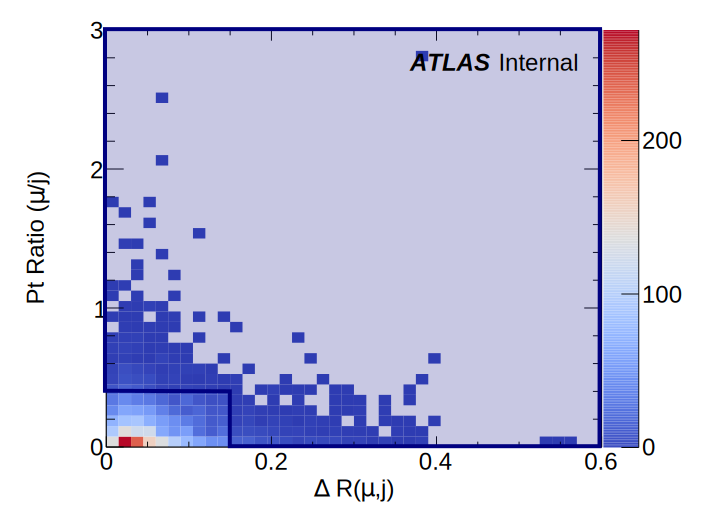
\includegraphics[width=.48\textwidth]{figs/ssww_13tev/custom_or/sig_Muon_DR_PtRatio_edited}
  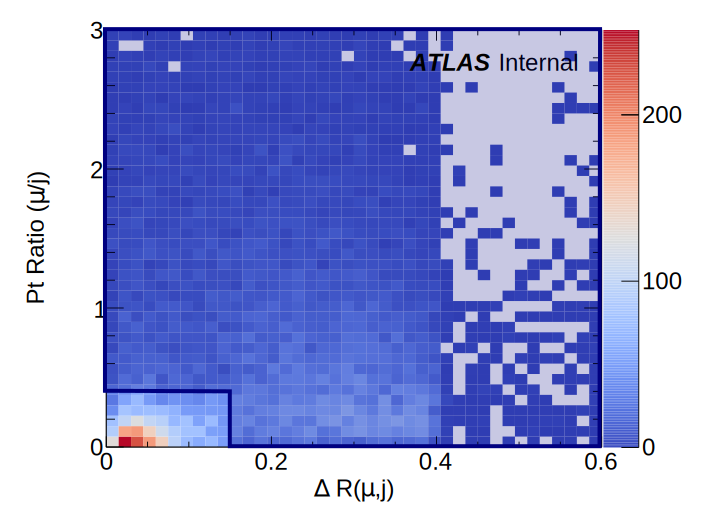
\includegraphics[width=.48\textwidth]{figs/ssww_13tev/custom_or/bkg_Muon_DR_PtRatio_edited}
  \caption{Two-dimensional plots of $\ptratio(\mu,j)$ vs $\deltar(\mu,j)$ for truth-matched third muons in events that pass the trilepton veto for EWK and QCD \ssww signal (left) and $WZ$ background (right).  The blue overlay indicates the area in which the third leptons will pass the custom OR and result in the event failing the trilepton veto.}
  \label{fig:ssww13tev_customor_muon_2d}
\end{figure}

Tests of the performance of the Custom OR yield promising results, with approximately 20\% reduction in $WZ$ background compared to less than 2\% signal loss in the signal region.
Unfortunately, due to differences between the primary analysis framework and the one used for testing, in practice the gains in $WZ$ rejection are not nearly as substantial, and ultimately the Custom OR is not included in the final analysis.
However, it is still a potentially useful tool for improving background rejection via lepton number vetoes in analyses with overly aggressive OR procedures.


\subsection{Estimation of the $V\gamma$ background}\label{ssww13tev:wgamma}

\subsection{Estimation of backgrounds from charge misidentification}\label{ssww13tev:charge_misid}
%\TODO{Brief overview of charge misID handling.  I didn't work on this either, but if i recall it was more involved than other backgrounds so it probably deserves its own section. This probably doesn't need to be too long, just explain the method and maybe throw in a plot of charge misID rates.  I think there are some good plots in the APS talk I gave.}

If an electron's charge is mis-reconstructed, it can lead to a real, opposite-sign lepton pair passing the same-sign requirement in the event selection.
There are two primary reasons this can occur:
\begin{enumerate}
\item An electron emits a photon via bremsstrahlung which then converts into an electron-positron pair, and the conversion track with the wrong electric charge is matched to the original electron.
This is the dominant process leading to charge flip, and it is highly dependent on the electron $\eta$ due to the different amount of detector material the electron passes through.
\item The curvature of the electron's track is mismeasured, resulting in the wrong charge being assigned.
This process is dependent on the momentum of the electron, as its track becomes more straight as the momentum of the electron increases.
\end{enumerate}

In order to estimate this background, the rate at which an electron's charge is misidentified is calculated from $Z\rightarrow e^{+}e^{-}$ MC simulation.
It is known that the MC does not perfectly model the material effects leading to charge flip; as a result, scale factors are applied to the MC in order for it to to better reflect the real performance.
These scale factors are obtained from the ratio of data and uncorrected MC charge mis-ID rates in~\cite{2018.ssww-13tev-atlas-support} following the method outlined in~\cite{2017.charge-flip-support}.
Once the scale factors are applied, the charge misidentification rate $\varepsilon$ can be extracted by comparing the electron's reconstructed charge with the charge of its truth particle:
\begin{equation}
  \varepsilon(\eta,\pt) = \frac{N_{\textrm{wrong\ charge}}}{N_{\textrm{prompt\ electrons}}}
\end{equation}
The charge mis-ID rate is calculated in bins of electron $|\eta|$ and $\pt$ and varies from below $0.1\%$ in the central region of the detector up to $8\%$ in the forward regions for high $\pt$ (above $90\gev$) electrons.
A two-dimensional plot of $\varepsilon$ can be found in Figure~\ref{fig:charge_flip_rates}.

\begin{figure}
  \centering
  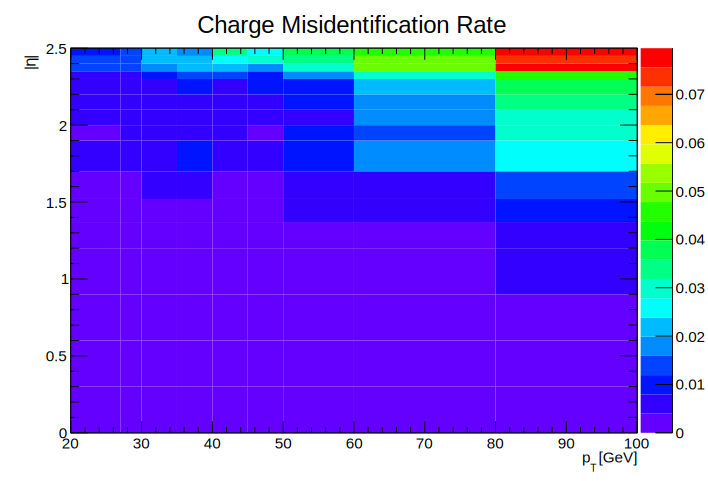
\includegraphics[width=.75\textwidth]{figs/ssww_13tev/backgrounds/charge_flip/charge_flip_2d}
  \caption{Charge misidentification rates for electrons as a function of $|\eta|$ and $\pt$.  Rates are calculated from $Z\rightarrow e^{+}e^{-}$ MC after applying sacle factors to approximate the charge mis-ID rates in data.}
  \label{fig:charge_flip_rates}
\end{figure}

%The size of the charge mis-ID background in a given region (signal or control region) is estimated from events that pass the region's default event selection but with an opposite-sign lepton pair.
Given the charge flip rate $\varepsilon(\eta,\pt)$, the rate at which an electron has its charge correctly reconstructed is $(1-\varepsilon)$.
Thus there are three possible combinations of charge identification, assuming a two-electron event:
\begin{enumerate}
\item Both electrons are reconstructed correctly: $(1-\varepsilon)^2$
\item Both electrons are mis-reconstructed: $\varepsilon^2$
\item Only one electron is mis-reconstructed: $2\varepsilon(1-\varepsilon)$
\end{enumerate}

In order to estimate the size of the background from charge misidentification, opposite-sign events are selected using the default event selection for a given signal or control region with the same-sign requirement inverted.
These events are then weighted by the probability for one of the electrons to be reconstructed with the wrong charge:
\begin{equation}
\omega = \frac{\varepsilon_1(1-\varepsilon_2)+\varepsilon_2(1-\varepsilon_1)}{(1-\varepsilon_1)(1-\varepsilon_2)+\varepsilon_1\varepsilon_2}
\label{ssww13tev:ch_flip_weight}
\end{equation}
%\begin{equation}
%\omega = \frac{\varepsilon_1(1-\varepsilon_2)+\varepsilon_2(1-\varepsilon_1)}{1-(\varepsilon_1+\varepsilon_2)+2\varepsilon_1\varepsilon_2}
%\label{ssww13tev:ch_flip_weight2}
%\end{equation}
where the subscripts 1 and 2 refer to the leading and subleading electrons, respectively, and $\varepsilon_i$ is a function of the $\eta$ and $\pt$ of the $i^{\textrm{th}}$ electron.
In the case of an event with only one electron and one muon, Equation~\ref{ssww13tev:ch_flip_weight} simplifies:
\begin{equation}
\omega = \frac{\varepsilon}{1-\varepsilon}
\end{equation}
This method assumes that there is little contamination from fake electrons in the opposite-sign sample, and this has been verified with MC simulation.

Additionally, charge-flipped electrons tend to be reconstructed with lower energy when compared to electrons with the correct charge.
This is due to energy loss from the material interactions that can cause the charge to be misidentified.
A correction factor is calculated from MC simulations, comparing the $\pt$ of the truth electron to its reconstructed counterpart:
\begin{equation}
\alpha = \frac{\Big(\frac{\pt^{\textrm{reco}}}{\pt^{\textrm{truth}}}-1\Big)_{\textrm{correct charge}}}{\Big(\frac{\pt^{\textrm{reco}}}{\pt^{\textrm{truth}}}-1\Big)_{\textrm{wrong charge}}}
\label{ssww13tev:ch_flip_alpha}
\end{equation}
The correction is then applied to the $\pt$ of the charge-flipped electron via
\begin{equation}
\pt = \pt^0/(1+\alpha)+dE
\label{ssww13tev:ch_flip_energy_corr}
\end{equation}
where $\pt^0$ is the uncorrected $\pt$ of the electron and $dE$ is a gaussian smearing factor centered at zero with a width related to the energy resolution.
Since which electron is misreconstructed is never determined in this method, in the case of a two-electron event, the energy correction is applied randomly to one of the two electrons based on the probabilities for them to be charge-flipped.
This also determines the overall sign of the event; the charge of the electron that does not recieve the correction is taken to be the charge for both.

Systematic uncertainties on the charge mis-ID rates are calculated by generating two additional sets of rates with the uncertainties on the scale factors varied up and down.
The size of the estimated charge flip background without the energy correction applied is also taken as a systematic uncertainty.
These systematic uncertainties are estimated to be approximately $\pm 15\%$.

\subsubsection{Validation of the charge misidentification estimate}\label{ssww13tev:ssincl_vr}
%The performance of the charge misidentification estimation is tested in $e^{\pm}e^{\pm}$ events with a di-electron invariant mass that lies within $15\gev$ of the $Z$ boson mass.
%Disagreements between data and background at high $\pt$ and $\eta$ have been found to be due to backgrounds from misidentified leptons, which are not included due to unreliable modeling in this particular region.

The performance of the charge misidentification estimation is tested in the same-sign inclusive validation region (VR), defined in Table~\ref{tab:ssww13tev_ssincl_vr_def}.
For $ee$ events, the mass of the dilepton pair is required to lie within $15\gev$ of the $Z$ boson mass to increase the purity of the charge flip background.
$t\bar{t}$ production, which can contribute to both the charge mis-ID and fake lepton backgrounds, is suppressed by the $b$-jet veto.
The di-electron invariant mass is shown in Figure~\ref{fig:ssww13tev_ssincl_mll}, and distributions of the leading and subleading electron $\pt$ in the $ee$-channel are shown in Figure~\ref{fig:ssww13tev_ssincl_ptlep} with the $Z$ mass cut inverted.
Agreement between data and prediction is seen within the total statistical and systematic uncertainties in the VR.

\begin{table}[htbp]
  \centering
  \begin{tabular}{c}
    Same-sign inclusive VR \\
    \hline\hline
    Exactly 2 same-sign signal leptons\\
    $\pt > 27\gev$ for both leptons \\
    $m_{ll} > 20\gev$\\
    $|m_{ee} - m_Z| > 15\gev$ ($ee$-channel only) \\
    $N_{b\textrm{-jet}} = 0$\\
    \hline
  \end{tabular}
  \caption{Selection criteria for the same-sign inclusive validation region.}
  \label{tab:ssww13tev_ssincl_vr_def}
\end{table}

\begin{figure}
  \centering
  \includegraphics[width=.48\textwidth]{figs/ssww_13tev/backgrounds/charge_flip/ee-CutCRInclusiveSSZ-Mll_Zpeak-lin}
  \caption{Dilepton invariant mass distribution $m_{ll}$ for the $ee$ channel in the same-sign inclusive VR.}
  \label{fig:ssww13tev_ssincl_mll}
\end{figure}

\begin{figure}
  \centering
  \includegraphics[width=.48\textwidth]{figs/ssww_13tev/backgrounds/charge_flip/ee-CutCRInclusiveSSZVeto-l0_pt-lin.pdf}
  \includegraphics[width=.48\textwidth]{figs/ssww_13tev/backgrounds/charge_flip/ee-CutCRInclusiveSSZVeto-l1_pt-lin.pdf}
  \caption{$\pt$ distributions for the leading (left) and subleading (right) electron for the $ee$ channel in the same-sign inclusive VR.  In these plots, the cut requiring $m_{ee}$ to fall within the $Z$ mass window has been inverted in order to test the modelling away from the $Z$ peak.}
  \label{fig:ssww13tev_ssincl_ptlep}
\end{figure}

\subsection{Estimation of non-prompt backgrounds with the fake factor method}\label{ssww13tev:fake_factor}
Events with one prompt lepton produced in asociation with hadronic jets can pass the event selection if a jet is misidentified as a charged lepton or if a non-prompt lepton from the decay of a heavy flavor particle (such as $b$- and $c$-hadrons) passes the signal lepton criteria.
These misidentified jets and non-prompt leptons are collectively referred to as \emph{fake leptons}, or simply \emph{fakes}.
The rate at which a fake lepton is misidentified is generally not modelled well enough by the MC to accurately estimate their contributions directly from simulation.
Therefore, a data-driven technique called the \emph{fake factor} is used to estimate the size and shape of background processes from fake leptons.
In this analysis, a new modification to the fake factor is used involving the particle isolation variables; the method is outlined in the context of the \emph{default} fake factor in Section~\ref{ssww13tev:ff_method_default}, and the modified fake factor is outlined in Section~\ref{ssww13tev:ff_method_ptcone}.

%---------------------------------------------------------------------------------------------
%
%---------------------------------------------------------------------------------------------
\subsubsection{Overview of the default fake factor method}\label{ssww13tev:ff_method_default}
The goal of the fake factor method is to measure the fake rate from real collision events in a region enriched in fake leptons and use it to estimate the size of the fake lepton background in a chosen signal or control region.
This is done by creating two samples using different lepton definitions: 
\begin{enumerate}
\item The \emph{nominal} sample is made up of leptons passing the signal selection.
\item The \emph{loose} sample is made up of leptons that fail the signal selection while still passing a loosened set of criteria.  This sample is enriched in fake leptons and is orthogonal to the set of signal leptons.
\end{enumerate}
Using the sets of nominal and loose leptons, a fake factor $f$ can be calculated in a region enriched in processes that are prone to producing fake leptons:
\begin{equation}
f = \frac{N_{\textrm{nominal}}}{N_{\textrm{loose}}}
\label{eq:ssww13tev_ff_default_unbinned}
\end{equation}
Since the fake rate is not expected to be constant over the entire phase space, the fake factor can be divided into bins:
\begin{equation}
f(b) = \frac{N_{\textrm{nominal}}(b)}{N_{\textrm{loose}}(b)}
\label{eq:ssww13tev_ff_default_binned}
\end{equation}
where $b$ represents the bin number.
In this analysis, the fake factor is binned in lepton $\pt$.

In order to estimate the fake background contribution in a given signal or control region, the fake factor is applied to a second control region with a selection identical to the region of interest with one of the leptons required to satisfy the loose criteria.
The region for which the background is estimated contains two nominal leptons and is referred to as \emph{nominal+nominal} ($NN$), and the associated control region where the fake factor is applied contains one nominal and one loose lepton and is referred to as \emph{nominal+loose} ($NL$).
The fake background in a NN region can then be calculated as:
\begin{equation}
N_{NN}^{\textrm{fake\ bkg.}} = \sum\limits_{b}f(b) N_{NL}(b)
\label{eq:ssww13tev_ff_bkg_nosub}
\end{equation}

Backgrounds containing two prompt leptons can also enter the $NL$ region if one of the leptons passes the nominal selection and the other passes the loose selection.
Since the fake factor method estimates the fake background by scaling the amount of non-prompt events in the $NL$ region, if these prompt contributions are not be removed, they will be included in the scaling and the background will be overpredicted.
The final estimate of the fake background becomes:
\begin{equation}
N_{NN}^{\textrm{fake\ bkg.}} = \sum\limits_{b}f(b) \big(N_{NL}(b) - N_{NL}^{\textrm{prompt}}(b)\big)
\label{eq:ssww13tev_ff_bkg}
\end{equation}

%---------------------------------------------------------------------------------------------
%
%---------------------------------------------------------------------------------------------
\subsubsection{The fake factor with $\ptcone$}\label{ssww13tev:ff_method_ptcone}
When a jet produces a non-prompt lepton, that lepton only carries a fraction of the underlying jet's total momentum.
Due to the isolation cut applied to the nominal leptons, they typically carry a much larger percentage of the underlying jet momentum\footnote{Since the isolation variables are a measure of detector activity around the lepton, if other nearby particles carried a significant portion of the jet's momentum, the lepton would likely fail this cut.} than the loose leptons (which are allowed to fail this criteria).

This discrepancy in the underlying jet momentum fraction can cause problems in the calculation of the fake factor $f$.
Consider the case where two separate events have jets of identical momentum, but one produces a non-prompt lepton that passes the nominal selection, and the other produces a non-prompt lepton that passes the loose selection.
The loose lepton on average will have lower $\pt$ than the nominal lepton despite both originating from jets with the same momentum.
This can be seen explicitly when comparing the $\pt$ of a muon to its associated truth jet:
\begin{equation}
\Delta\pt(\mu,j) = \frac{\pt(j)-\pt(\mu)}{\pt(j)+\pt(\mu)}
\label{eq:ssww13tev_ff_deltapt}
\end{equation}
Since muons are not included in the jet reconstruction algorithm, $\Delta\pt$ approximates the momentum of the muon compared to the rest of the jet.
For muons that carry more than 50\% of the jet's momentum, $\Delta\pt$ will be negative and vice-versa.
The $\Delta\pt$ distributions for nominal and loose muons in $t\bar{t}$ MC events is shown Figure~\ref{fig:ssww13tev_ff_deltapt}, where a $50\gev$ jet on average corresponds to a $35\gev$ nominal muon and a $20\gev$ loose muon\footnote{To better illustrate the point, here the muon is added back into the jet $\pt$, and the corresponding muon $\pt$ is obtained via $\Delta\pt(\mu,j) = \frac{\big(\pt(j)-\pt{\mu}\big)-\pt(\mu)}{\big(\pt(j)-\pt(\mu)\big)+\pt(\mu)} = \frac{\pt(j)-2\pt(\mu)}{\pt(j)}$.}.

\begin{figure}[htbp]
  \centering
  \includegraphics[width=.6\textwidth]{figs/ssww_13tev/backgrounds/ff/deltapt_ttbar}
  \caption{$\Delta\pt$ distributions for nominal (blue) and loose (red) muons in simulated $t\bar{t}$ events.  Each muon has been matched to a truth-level jet.  Both distributions are normalized to unit area.}
  \label{fig:ssww13tev_ff_deltapt}
\end{figure}

Since the default fake factor defined in Equation~\ref{eq:ssww13tev_ff_default_binned} is binned in lepton $\pt$, within a given bin, the underlying jet $\pt$ spectrum can differ substantially between the numerator and the denominator.
Additionally, these differences can vary depending on the process producing the non-prompt leptons or on the specific kinematic selections of the signal or control regions where the fake factor is applied.

Fortunately, the majority of the jet momentum not carried by the non-prompt lepton (excluding neutrinos) can be recovered using isolation variables.
A track-based isolation is chosen, referred to as $\ptcone$, and it contains the sum of the $\pt$ of all particle tracks originating from the primary vertex within a cone of $\deltar < 0.3$ around the lepton.
Thus, the sample of loose leptons in the denominator of the fake factor calculation is binned in $\ptptcone$ rather than simply lepton $\pt$.
Adding the isolation cone greatly reduces the difference in the fraction of the underlying jet momentum carried by the nominal and loose leptons.
To check this, a new $\Delta\pt$ is calculated between a lepton and its matched truth jet, where the truth jet $\pt$ has been corrected to include all muons within a cone of $\deltar < 0.4$:
\begin{equation}
\pt(j) = \pt(j_{\textrm{truth}})+\sum\limits_{\deltar < 0.4}\pt(\mu_{\textrm{truth}})
\label{eq:ssww13tev_ff_jet_corr}
\end{equation}
The $\Delta\pt$ distributions comparing $\pt$ and $\ptptcone$ for nominal and loose leptons using the corrected jet $\pt$ are found in Figure~\ref{fig:ssww13tev_ff_deltapt_ptcone}, and better agreement is seen between the numerator (nominal) and denominator (loose with $\ptptcone$) distributions.

\begin{figure}[htbp]
  \centering
  \includegraphics[width=.6\textwidth]{figs/ssww_13tev/backgrounds/ff/dpt_muon_ttbar}\\
  \includegraphics[width=.6\textwidth]{figs/ssww_13tev/backgrounds/ff/dpt_elec_ttbar}
  \caption{$\Delta\pt$ distributions for muons (top) and electrons (bottom) in simulated $t\bar{t}$ events.  Each lepton has been matched to a truth-level jet, and that truth jet has had its $\pt$ corrected to include all truth muons within a cone of $\deltar < 0.4$.  The nominal leptons are in black. $\Delta\pt$ is calculated for the loose leptons using $\pt$ (red) and $\ptptcone$ (blue).}
  \label{fig:ssww13tev_ff_deltapt_ptcone}
\end{figure}

The numerator remains binned in lepton $\pt$, due to the fact that it is meant to mirror the signal region as closely as possible, and the signal lepton selection does not use $\ptptcone$.
The impact of this is expected to be negligible due to the $\ptcone$ isolation being small for signal leptons, as shown for muons in Figure~\ref{fig:ssww13tev_ff_ptcone_muons}.
Finally, the fake factor $f$ becomes:

\begin{equation}
%f_b = \frac{N_{\textrm{nominal}}^b(\pt)}{N_{\textrm{loose}}^b(\ptptcone)}
f(b) = \frac{N_{\textrm{nominal}}\big(b(\pt)\big)}{N_{\textrm{loose}}\big(b(\ptptcone)\big)}
\label{eq:ssww13tev_ff_ptcone_binned}
\end{equation}

\begin{figure}[htbp]
  \centering
  \includegraphics[width=.6\textwidth]{figs/ssww_13tev/backgrounds/ff/ptcone_muon_ttbar}
  \caption{Distributions of $\ptcone/\pt$ for nominal (black) and loose (red) muons in simulated $t\bar{t}$ events.}
  \label{fig:ssww13tev_ff_ptcone_muons}
\end{figure}

%---------------------------------------------------------------------------------------------
%
%---------------------------------------------------------------------------------------------
\subsubsection{Application of the fake factor}\label{ssww13tev:ff_implementation}
The fake factor itself is measured from a sample data events passing a dijet selection requiring exactly one lepton (either passing the nominal or loose selections) and at least one jet.
The leading jet must also be $b$-tagged and approximately back-to-back with the lepton in order to enhance non-prompt lepton contributions while reducing contributions from processes involving $W$ and $Z$ bosons.
$W$ boson events are further suppressed by requiring the sum of the $\met$ and the transverse mass of the lepton and $\met$ to be less than $50\gev$.
The full event selection for the dijet region is summarized in Table~\ref{tab:ssww13tev_dijet_cr}.

\begin{table}[hbtp]
  \centering
  \begin{tabular}{c}
    Dijet event selection \\
    \hline\hline
    Event preselection\\
    Exactly one lepton with $\pt > 15\gev$\\
    $N_{\textrm{jet}} > 0$ \\
    Leading jet is $b$-tagged \\
    $\pt^{\textrm{lead.\ jet}} > 25\gev$\\
    $\pt^{\textrm{lead.\ jet}} > 30\gev$ if $|\eta_j| > 2.5$ \\
    $|\Delta\phi(l,\textrm{lead.\ jet})| > 2.8$ \\
    $m_{\textrm{T}}(l,\met) + \met < 50\gev$ \\
    \hline
  \end{tabular}
  \caption{Event selection for the dijet region used for calculating the fake factor. The selected lepton can pass either the nominal (signal) or loose selections.  In the case of the nominal leptons, the $\pt > 27\gev$ requirement is replaced with $\pt > 15\gev$.}
  \label{tab:ssww13tev_dijet_cr}
\end{table}

The numerator sample is constructed from dijet events in which the lepton passes the nominal (signal) selection and is binned in the lepton $\pt$.
Similarly, the denominator sample is made up of the remaining dijet events where the lepton passes the loose selection and is binned in the lepton $\ptptcone$.
The nominal and loose leptons pass the signal selection\footnote{The $\pt > 27\gev$ cut in the signal lepton selection is dropped in favor of the $\pt > 15\gev$ requirement in the dijet selection.} and loose selection, respectively, defined earlier in Table~\ref{tab:ssww13tev_muon_selection} for muons and Table~\ref{tab:ssww13tev_elec_selection} for electrons.
Backgrounds from $W$+jets, $Z$+jets, $t\bar{t}$, and single top processes are estimated from MC simulations requiring one lepton to be prompt using the truth information; these contributions are subtracted from the dijet data.
The fake factor is then calculated using Equation~\ref{eq:ssww13tev_ff_ptcone_binned} for muons and for central and forward electrons separately.
The muon fake factor is shown in Figure~\ref{fig:ssww13tev_ff_muon}, and the two electron fake factors are shown in Figure~\ref{fig:ssww13tev_ff_elec}.
The numerical values of the fake factors, including their systematic uncertainties which will be discussed in Section~\ref{ssww13tev:ff_systematics}, are listed in Table~\ref{tab:ssww13tev_ff}.

\begin{figure}[htbp]
  \centering
  \includegraphics[width=.6\textwidth]{figs/ssww_13tev/backgrounds/ff/muon_ff}
  \caption{The measured fake factor as a function of muon $\ptptcone$.  The error bars represent the statistical uncertainty only.}
  \label{fig:ssww13tev_ff_muon}
\end{figure}

\begin{figure}[htbp]
  \centering
  \includegraphics[width=.6\textwidth]{figs/ssww_13tev/backgrounds/ff/elec_ff}
  \caption{The measured fake factor as a function of electron $\ptptcone$ in the central ($|\eta|<1.37$, blue) and forward ($|\eta| > 1.37$, red) regions of the detector.  The error bars represent the statistical uncertainty only.}
  \label{fig:ssww13tev_ff_elec}
\end{figure}

In order to properly account for the denominator being binned in $\ptptcone$, special care needs to be taken when estimating the fake background from the $NL$ regions.
For the purposes of the fake factor calculation, it is perhaps more intuitive to consider a loose \emph{object} with $\pt=\ptptcone$ instead of simply a loose \emph{lepton}, as the lepton and the underlying jet are treated as a whole with this method.
When the lepton $\pt$ cuts required by a particular signal or control region are applied to nominal and loose leptons, the cut is applied to the $\pt$ of the nominal lepton and to the $\ptptcone$ of the loose object.
Similarly, when looking up the fake factor weight for a given $NL$ event, the value taken from the bin corresponding to the $\ptptcone$ of the loose object.
Finally, when applying the weight to the event, $\ptptcone$ is assigned as the $\pt$ of the loose object.
Figure~\ref{fig:ssww13tev_ff_application} contains a graphical representation of this procedure.

\begin{figure}[htbp]
  \centering
  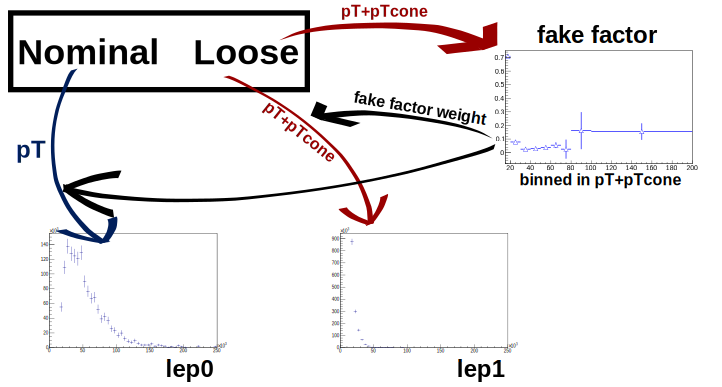
\includegraphics[width=.95\textwidth]{figs/ssww_13tev/backgrounds/ff/apply_ff}
  \caption{Graphical representation of the fake factor application using $\ptptcone$.  The value of $\ptptcone$ for the loose lepton is used to ``look up'' the fake factor weight which is then applied to the event.  The loose lepton's $\pt$ becomes $\ptptcone$ for the purpose of the fake background estimation.}
  \label{fig:ssww13tev_ff_application}
\end{figure}

Finally, it should be noted that the addition of $\ptcone$ to the loose object may cause the loose leptons in the denominator sample to migrate into higher bins.
This results in an overall decrease in the number of loose objects in the lower $\ptptcone$ bins due to there not being additional leptons at lower $\pt$ to replace them.
Since the fake factor is a ratio of the number of events in a bin, this effect causes the first few bins of the fake factor to increase, as can be seen clearly in Figure~\ref{fig:ssww13tev_ff_muon}.
However, the signal and control regions (and their corresponding $NL$ regions) contain a $\pt > 27\gev$ cut that prevents these migrations from negatively impacting the fake estimation.

%---------------------------------------------------------------------------------------------
%
%---------------------------------------------------------------------------------------------
\subsubsection{Systematic uncertainties}\label{ssww13tev:ff_systematics}
Four sources of systematic uncertainty are considered: the dijet event selection, the prompt background subtraction, the jet flavor composition, and residual dependence on the underlying jet $\pt$ spectrum.
In order to measure the impact of these systematics, new fake factors are computed with each of the systematic variations and the differences from the nominal values are taken as the uncertainty.
\begin{enumerate}
\item In order to estimate uncertainties due to the dijet selection, the cut on $M_{\textrm{T}}+\met$ is varied by $\pm5\gev$, $\Delta\phi(l,j)$ by $\pm 0.1$, and the jet $\pt$ cut by $+5\gev$.
\item To estimate the systematic uncertainty on the prompt background subtraction, the MC prediction in a $W$+jets control region is compared to data.  The discrepancy between data and MC is found to be approximately 10\%~\cite{2018.ssww-13tev-atlas-support}.  Therefore, the prompt background used for the subtraction is scaled up and down by $\pm 10\%$.
\item The difference in the jet flavor composition between the dijet events and the events in the $NL$ regions can affect the accuracy of the fake background estimation.  The dijet sample is dominated by light jets, while the $NL$ regions tend to be dominated by heavy flavor from $t\bar{t}$.  To account for this, the fake factor is computed with a $b$-jet veto.
\item To measure any residual dependence on the underlying jet $\pt$ spectrum, the leading jet $\pt$ distribution is reweighted to match the $\pt$ spectrum of truth jets that produce fake leptons in MC simulations.  This results in an increase in the number of nominal and loose leptons at high momentum~\cite{2018.ssww-13tev-atlas-support}.
\end{enumerate}
%An overall uncertainty of 50\% is assigned to the fake background estimation in $\mu^{\pm}\mu^{\pm}$ events, and between 40\% to 90\% for $e^{\pm}e^{\pm}$ and $\mu^{\pm}e^{\pm}$ events, including both statistical and systematic effects.

\begin{figure}[htbp]
  \centering
  \includegraphics[width=.6\textwidth]{figs/ssww_13tev/backgrounds/ff/muon_ff_sys}
  \caption{Systematic variations in the fake factor as a function of muon $\ptptcone$.  The individual fake factors obtained for each systematic variation are displayed with their statistical uncertainties.}
  \label{fig:ssww13tev_ff_muon_sys}
\end{figure}

\begin{figure}[htbp]
  \centering
  \includegraphics[width=.6\textwidth]{figs/ssww_13tev/backgrounds/ff/elec_central_ff_sys}\\
  \includegraphics[width=.6\textwidth]{figs/ssww_13tev/backgrounds/ff/elec_forward_ff_sys}
  \caption{Systematic variations in the fake factor as a function of electron $\ptptcone$ in the central ($|\eta|<1.37$, top) and forward ($|\eta| > 1.37$, bottom) regions of the detector.  The individual fake factors obtained for each systematic variation are displayed with their statistical uncertainties.}
  \label{fig:ssww13tev_ff_elec_sys}
\end{figure}

\begin{table}[hbtp]
  \begin{subtable}{\linewidth}
  \centering
  \resizebox{1.0\textwidth}{!}{
  \begin{tabular}{l|cccccccc}
    fake-factor & $\pt$  [15, 20]      &  $\pt$[20, 27]       &    $\pt$[27, 35]     &    $\pt$[35, 45]     &    $\pt$[45, 55]     &    $\pt$[55, 65]     &    $\pt$[65, 75]     &    $\pt$[75, 200]    \\ \hline\hline
    nominal     & 0.649 $\pm$ 0.007  & 0.083 $\pm$ 0.002 & 0.024 $\pm$ 0.002  & 0.021 $\pm$ 0.003   & 0.044 $\pm$ 0.007   & 0.067 $\pm$ 0.018  & 0.160 $\pm$ 0.055   & 0.481 $\pm$ 0.088 \\ \hline
    \multirow{2}{*}{MT+MET}   & 0.649 $\pm$ 0.007  & 0.082 $\pm$ 0.002   & 0.082 $\pm$ 0.002    & 0.020 $\pm$ 0.003    & 0.045 $\pm$ 0.007 & 0.068 $\pm$ 0.018 & 0.207 $\pm$ 0.062 & 0.523 $\pm$ 0.086 \\
    & 0.648 $\pm$ 0.007 & 0.083 $\pm$ 0.003 & 0.024 $\pm$ 0.002 & 0.022 $\pm$ 0.004 & 0.044 $\pm$ 0.007 & 0.054 $\pm$ 0.020 & 0.207 $\pm$ 0.060 & 0.389 $\pm$ 0.081 \\ \hline
    \multirow{2}{*}{$\Delta\phi(\ell,j)$}    & 0.645 $\pm$ 0.008 & 0.083 $\pm$ 0.003 & 0.024 $\pm$ 0.002 & 0.021 $\pm$ 0.004 & 0.045 $\pm$ 0.008 & 0.064 $\pm$ 0.021 & 0.064 $\pm$ 0.058 & 0.438 $\pm$ 0.092 \\
      & 0.646 $\pm$ 0.006 & 0.083 $\pm$ 0.002 & 0.024 $\pm$ 0.002 & 0.020 $\pm$ 0.003 & 0.043 $\pm$ 0.006 & 0.076 $\pm$ 0.017 & 0.174 $\pm$ 0.050 & 0.448 $\pm$ 0.078 \\ \hline
    Jet $\pt$        & 0.650 $\pm$ 0.007 & 0.083 $\pm$ 0.002 & 0.024 $\pm$ 0.002 & 0.021 $\pm$ 0.003 & 0.045 $\pm$ 0.007 & 0.069 $\pm$ 0.018 & 0.159 $\pm$ 0.018 & 0.481 $\pm$ 0.088 \\ \hline 
    $N_{\textrm{b-jet}} = 0$      & 0.724 $\pm$ 0.003 & 0.094 $\pm$ 0.001 & 0.035 $\pm$ 0.001 & 0.025 $\pm$ 0.002 & 0.022 $\pm$ 0.004 & 0.060 $\pm$ 0.015 & 0.026 $\pm$ 0.053 & 0.044 $\pm$ 0.134 \\ \hline 
    \multirow{2}{*}{Bkg. subtraction}   & 0.648 $\pm$ 0.007 & 0.083 $\pm$ 0.002 & 0.024 $\pm$ 0.002 & 0.019 $\pm$ 0.003 & 0.037 $\pm$ 0.007 & 0.044 $\pm$ 0.019 & 0.096 $\pm$ 0.062 & 0.370 $\pm$ 0.082 \\
    & 0.649 $\pm$ 0.007 & 0.083 $\pm$ 0.002 & 0.025 $\pm$ 0.002 & 0.022 $\pm$ 0.003 & 0.050 $\pm$ 0.007 & 0.090 $\pm$ 0.017 & 0.224 $\pm$ 0.052 & 0.591 $\pm$ 0.099 \\ \hline 
   Jet $\pt$ Reweight & 0.539 $\pm$ 0.077 & 0.093 $\pm$ 0.007 & 0.025 $\pm$ 0.004 & 0.043 $\pm$ 0.019 & 0.063 $\pm$ 0.014 & 0.085 $\pm$ 0.025 & 0.141 $\pm$ 0.110 & 1.962 $\pm$ 0.492 \\ 
    \hline
  \end{tabular}
  }
  \caption{Fake-factor values for muons.}
  \end{subtable}

  \vspace{10mm}

  \begin{subtable}{\linewidth}
  \centering
  \resizebox{1.0\textwidth}{!}{
  \begin{tabular}{l|cccccccc}
    fake-factor   &  $\pt$[20, 27]       &    $\pt$[27, 35]     &    $\pt$[35, 45]     &    $\pt$[45, 55]     &    $\pt$[55, 65]     &    $\pt$[65, 75]     &    $\pt$[75, 200]    \\ \hline\hline
    nominal     & 0.491 $\pm$ 0.031 & 0.140 $\pm$ 0.020 & 0.111 $\pm$ 0.023 & 0.256 $\pm$ 0.049 & 0.546 $\pm$ 0.091 & 0.460 $\pm$ 0.140 & 0.939 $\pm$ 0.125 \\ \hline
    \multirow{2}{*}{MT+MET}   & 0.493 $\pm$ 0.030 & 0.138 $\pm$ 0.019 & 0.115 $\pm$ 0.022 & 0.261 $\pm$ 0.045 & 0.559 $\pm$ 0.084 & 0.656 $\pm$ 0.091 & 0.802 $\pm$ 0.016 \\
                              & 0.488 $\pm$ 0.032 & 0.137 $\pm$ 0.020 & 0.110 $\pm$ 0.025 & 0.283 $\pm$ 0.053 & 0.503 $\pm$ 0.097 & 0.351 $\pm$ 0.149 & 1.117 $\pm$ 0.255 \\ \hline
    \multirow{2}{*}{$\Delta\phi(\ell,j)$}  & 0.489 $\pm$ 0.035 & 0.134 $\pm$ 0.021 & 0.105 $\pm$ 0.025 & 0.224 $\pm$ 0.048 & 0.593 $\pm$ 0.093 & 0.356 $\pm$ 0.144 & 0.928 $\pm$ 0.177 \\ 
     & 0.506 $\pm$ 0.029 & 0.140 $\pm$ 0.018 & 0.111 $\pm$ 0.022 & 0.260 $\pm$ 0.046 & 0.545 $\pm$ 0.084 & 0.546 $\pm$ 0.120 & 0.882 $\pm$ 0.103  \\  \hline
    Jet $\pt$    & 0.493 $\pm$ 0.032 & 0.146 $\pm$ 0.021 & 0.115 $\pm$ 0.024 & 0.259 $\pm$ 0.049 & 0.550 $\pm$ 0.091 & 0.460 $\pm$ 0.140 & 0.939 $\pm$ 0.125 \\ \hline 
    $N_{\textrm{b-jet}} = 0$      & 0.387 $\pm$ 0.009 & 0.130 $\pm$ 0.008 & 0.321 $\pm$ 0.012 & 0.473 $\pm$ 0.015 & 0.716 $\pm$ 0.180 & 0.716 $\pm$ 0.180 & 0.716 $\pm$ 0.180 \\ \hline 
    \multirow{2}{*}{Bkg. subtraction}   & 0.488 $\pm$ 0.031 & 0.138 $\pm$ 0.020 & 0.106 $\pm$ 0.023& 0.248 $\pm$ 0.049 & 0.529 $\pm$ 0.092 & 0.434 $\pm$ 0.143 & 0.888 $\pm$ 0.115 \\ 
      & 0.493 $\pm$ 0.031 & 0.142 $\pm$ 0.020 & 0.115 $\pm$ 0.023 & 0.264 $\pm$ 0.049 & 0.563 $\pm$ 0.090 & 0.485 $\pm$ 0.136 & 0.989 $\pm$ 0.132 \\  \hline
    Jet $\pt$ Reweight     & 0.445 $\pm$ 0.055 & 0.137 $\pm$ 0.037 & 0.065 $\pm$ 0.023 & 0.115 $\pm$ 0.033 & 0.603 $\pm$ 0.047 & 0.104 $\pm$ 0.105 & 0.299 $\pm$ 0.260 \\  
    \hline
  \end{tabular}}
  \caption{Fake-factor values for central electrons ($|\eta| < 1.37$).}
  \end{subtable}

  \vspace{10mm}

  \begin{subtable}{\linewidth}
  \centering
  \resizebox{1.0\textwidth}{!}{
  \begin{tabular}{l|cccccccc}
    fake-factor   &  $\pt$[20, 27]       &    $\pt$[27, 35]     &    $\pt$[35, 45]     &    $\pt$[45, 55]     &    $\pt$[55, 65]     &    $\pt$[65, 75]     &    $\pt$[75, 200]    \\ \hline \hline
    nominal     & 0.487 $\pm$ 0.046 & 0.148 $\pm$ 0.031  & 0.253 $\pm$ 0.046  & 0.412 $\pm$ 0.071  & 0.556 $\pm$ 0.117 & 0.691 $\pm$ 0.117 & 1.340 $\pm$ 0.340 \\ \hline   
 \multirow{2}{*}{MT+MET}   & 0.483 $\pm$ 0.045 & 0.152 $\pm$ 0.031 & 0.241 $\pm$ 0.043 & 0.443 $\pm$ 0.070 & 0.565 $\pm$ 0.106 & 0.668 $\pm$ 0.117 & 1.075 $\pm$ 0.189 \\ 
    & 0.495 $\pm$ 0.047 & 0.156 $\pm$ 0.033 & 0.271 $\pm$ 0.052 & 0.364 $\pm$ 0.074 & 0.664 $\pm$ 0.107 & 0.749 $\pm$ 0.056 & 0.885 $\pm$ 0.084 \\ \hline
    \multirow{2}{*}{$\Delta\phi(\ell,j)$}    & 0.471 $\pm$ 0.051 & 0.158 $\pm$ 0.035 & 0.247 $\pm$ 0.051 & 0.474 $\pm$ 0.085 & 0.283 $\pm$ 0.107 & 0.546 $\pm$ 0.149 & 1.189 $\pm$ 0.266 \\ 
      & 0.478 $\pm$ 0.042 & 0.170 $\pm$ 0.031 & 0.274 $\pm$ 0.046 & 0.389 $\pm$ 0.066 & 0.645 $\pm$ 0.104 & 0.757 $\pm$ 0.102 & 1.319 $\pm$ 0.326 \\ \hline
    Jet $\pt$   & 0.523 $\pm$ 0.048 & 0.149 $\pm$ 0.033 & 0.235 $\pm$ 0.045 & 0.429 $\pm$ 0.073 & 0.555 $\pm$ 0.117 & 0.691 $\pm$ 0.117 & 1.340 $\pm$ 0.340 \\ \hline
    $N_{\textrm{b-jet}} = 0$       & 0.525 $\pm$ 0.011 & 0.234 $\pm$ 0.013 & 0.644 $\pm$ 0.016 & 0.710 $\pm$ 0.014 & 0.274 $\pm$ 0.316 & 0.274 $\pm$ 0.316 & 0.274 $\pm$ 0.316 \\ \hline 
    \multirow{2}{*}{Bkg. subtraction}   & 0.484 $\pm$ 0.046 & 0.146 $\pm$ 0.031 & 0.248 $\pm$ 0.046 & 0.406 $\pm$ 0.071 & 0.545 $\pm$ 0.118 & 0.676 $\pm$ 0.118 & 1.317 $\pm$ 0.337 \\
    & 0.489 $\pm$ 0.046 & 0.151 $\pm$ 0.031 & 0.257 $\pm$ 0.046& 0.419 $\pm$ 0.071 & 0.568 $\pm$ 0.117 & 0.705 $\pm$ 0.115 & 1.363 $\pm$ 0.342 \\    \hline  
    Jet $\pt$ Reweight  & 0.328 $\pm$ 0.068 & 0.124 $\pm$ 0.048 & 0.297 $\pm$ 0.100 & 0.234 $\pm$ 0.061 & 0.680 $\pm$ 0.092 & 0.452 $\pm$ 0.138 & 2.385 $\pm$ 1.729 \\
 \hline
  \end{tabular}}
  \caption{Fake-factor values for forward electrons ($1.37 < |\eta|$).}
  \end{subtable}

  \caption{Values of the fake-factor in each $\pt$ bin and for each individual systematic source.}
  \label{tab:ssww13tev_ff}
\end{table}


%---------------------------------------------------------------------------------------------
%
%---------------------------------------------------------------------------------------------
\subsubsection{Results of the fake factor}\label{ssww13tev:ff_results}
The fake background contribution in the signal region is estimated by applying the fake factors to the equivalent $NL$ region using Equation~\ref{eq:ssww13tev_ff_bkg}, where the fake factor used corresponds to the flavor of the loose lepton in the event.
As usual, the prompt background is subtracted from the $NL$ events using MC simulation.
Charge misidentification is handled using the same method as in Section~\ref{ssww13tev:charge_misid}, with an additional set of charge flip rates calculated for loose leptons.
The fake background yields in the signal region are listed in Table~\ref{tab:ssww13tev_ff_signal_region}.
An overall uncertainty of 50\% is assigned to the fake background estimation in $\mu^{\pm}\mu^{\pm}$ events, and between 40\% to 90\% for $e^{\pm}e^{\pm}$ and $\mu^{\pm}e^{\pm}$ events, including both statistical and systematic effects.

\begin{table}[hbtp]
\centering
  \resizebox{\textwidth}{!}{
  \begin{tabular}{ l | r| r  r  r  r |r  r  r  r }
  & estimated yield & $f_e$ stat.\ up & $f_e$ stat.\ dn & $f_e$ syst.\ up & $f_e$ syst.\ dn & $f_\mu$ stat.\ up & $f_\mu$ stat.\ dn & $f_\mu$ syst.\ up & $f_\mu$ syst.\ dn\\
\hline\hline
$\ee$ & $11.42\pm 3.13$ & $1.69$ & $-1.69$ & $1.67$ & $-5.56$ & --- & --- & --- & ---\\
%\hline
$\mm$ & $4.82\pm 0.77$ & ---  & ---  & ---  & ---  & $0.65$ & $-0.65$ & $3.64$ & $-0.61$\\
%\hline
$\me$ & $37.08\pm 5.16$ & $4.90$ & $-4.90$ & $5.59$ & $-14.34$ & $1.39$ & $-1.39$ & $16.10$ & $-1.98$\\
\hline
\end{tabular}
}
\caption{Estimated yields for the fake lepton background. The estimated yield is shown in the first column together with the statistical uncertainty followed by the systematic uncertainties from variations of the the fake factors within their statistical (stat.) and systematic (syst.) uncertainties. The labels $f_e$ and $f_\mu$ indicate the fake factors for electrons and muons, respectively.}
  \label{tab:ssww13tev_ff_signal_region}
\end{table}

\subsubsection{Validation of the fake factor}\label{ssww13tev:ff_vr}
The accuracy of the fake factor method is tested in several validation regions, the most sensitive of which is the same-sign top fakes VR (SS top VR), defined in Table~\ref{tab:ssww13tev_topfakes_vr_def}.
This region inverts the signal region's $b$-jet veto to accept events with exactly one $b$-jet.
Due to this requirement, the dominant source of events comes from the $t\bar{t}$ process where a $b$-jet fakes an isolated lepton.
The distribution of the subleading lepton $\pt$ in this VR is shown in Figure~\ref{fig:ssww13tev_ff_fakes_vr} for all lepton flavor combinations.
There is good agreement between the data and the prediction, even when only taking into account the statistical uncertainty and not the large systematic uncertainties assigned to the fake estimation.
%The subleading lepton is most likely to be the fake.

\begin{table}[htbp]
  \centering
  \begin{tabular}{c}
    Same-sign inclusive VR \\
    \hline\hline
    Exactly 2 same-sign signal leptons\\
    $\pt > 27\gev$ for both leptons \\
    $m_{ll} > 20\gev$\\
    $|m_{ee} - m_Z| > 15\gev$ ($\ee$-channel only) \\
    $N_{b\textrm{-jet}} = 1$\\
    $N_{\textrm{jet}} \ge 2$ \\
    Leading jet $\pt > 65\gev$ \\
    Subleading jet $\pt > 35\gev$ \\
    \hline
  \end{tabular}
  \caption{Selection criteria for the same-sign top fakes validation region.}
  \label{tab:ssww13tev_topfakes_vr_def}
\end{table}

\begin{figure}
  \centering
  \includegraphics[width=.48\textwidth]{figs/ssww_13tev/backgrounds/ff/fakes_vr/mm-CutCRTopFakesSSZVeto-l1_pt-lin}
  \includegraphics[width=.48\textwidth]{figs/ssww_13tev/backgrounds/ff/fakes_vr/ee-CutCRTopFakesSSZVeto-l1_pt-lin}\\
  \includegraphics[width=.48\textwidth]{figs/ssww_13tev/backgrounds/ff/fakes_vr/emme-CutCRTopFakesSSZVeto-l1_pt-lin}
  \includegraphics[width=.48\textwidth]{figs/ssww_13tev/backgrounds/ff/fakes_vr/ll-CutCRTopFakesSSZVeto-l1_pt-lin}
  \caption{Distributions of the subleading lepton $\pt$ in the same-sign top fakes VR for  $\mm$ events (top right), $\ee$ events (top left), $\me$ events (bottom left), and all events combined (bottom right).  All errors are statistical only.}
  \label{fig:ssww13tev_ff_fakes_vr}
\end{figure} 

